\documentclass[12pt]{article}
\usepackage[T2A]{fontenc}
\usepackage[utf8]{inputenc}
\usepackage{multirow}
\usepackage{caption}
\usepackage{subcaption}
\usepackage{amsmath}
\usepackage{changepage}
\usepackage{graphicx}
\usepackage{float}
\usepackage[english,russian]{babel}
\usepackage{amsmath, amsfonts, amssymb, amsthm, mathtools}
\usepackage{xcolor}
\usepackage{array}
\usepackage{hyperref}
\usepackage{icomma}
\usepackage{mathtext} 
\usepackage[top = 1.5cm, left = 1.5 cm, right = 1.5 cm, bottom = 3 cm]{geometry}
\graphicspath{ {./images/} }
 
\title{Резонанс токов в параллельном контуре.}
\author{Шахматов Андрей, Б02-304}
\date{\today}
  
\begin{document}
\begin{titlepage}
    \begin{center}
        {\large МОСКОВСКИЙ ФИЗИКО-ТЕХНИЧЕСКИЙ ИНСТИТУТ (НАЦИОНАЛЬНЫЙ ИССЛЕДОВАТЕЛЬСКИЙ УНИВЕРСИТЕТ)}
    \end{center}
    \begin{center}
        {\large Физтех-школа физики и исследований им. Ландау}
    \end{center}


    \vspace{3cm}
    {\huge
        \begin{center}
            \textbf{Резонанс токов в параллельном контуре.}
        \end{center}
    }
    \vspace{2cm}
    \begin{flushright}
        {\LARGE Автор:\\ Шахматов Андрей Юрьевич \\
            \vspace{0.2cm}
            Б02-304}
    \end{flushright}
    \vspace{7 cm}
    \begin{center}
        Долгопрудный 2024
    \end{center}
    \thispagestyle{empty}
\end{titlepage}

% \maketitle

\begin{abstract}
    Исследованы резонансные значения частот переменного тока в парралельном контуре для различных
    значений ёмкости конденсатора. Измерена амплитудно-частотная и фазо-частотная характеристика контура.
    По полученным данным несколькими способами определена добротность контура и характеристики электрических элементов.
\end{abstract}

% \tableofcontents

\section{Введение}
Цель работы заключается в исследование резонанса токов в параллельном колебательном контуре с изменяемой ёмкостью, включающее получение амплитудно-частотных и фазово-частотных характеристик,
а также определение основных параметров контура.

\section{Методика}
В работе исследовалось поведение парралельного контура, схема которого представлена на Рис. \ref{pic:scheme}. 
Так как в реальности конденсаторы и катушки имеют активное сопростивление, реальную схему установки можно изобразить как показано 
на Рис. \ref{pic:scheme2}.

\begin{figure}[H]
    \centering
    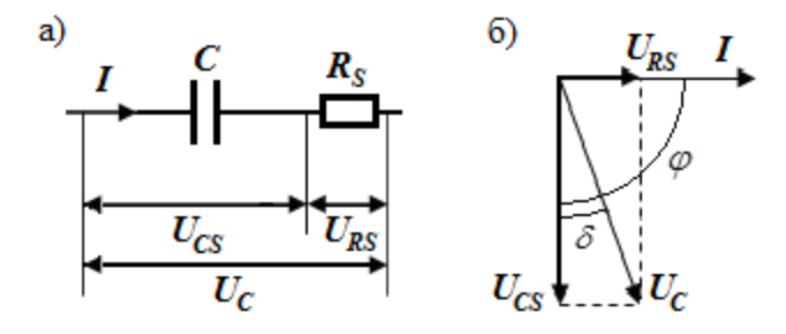
\includegraphics[width=0.4\textwidth]{im1.png}
    \caption{Схема установки.}
    \label{pic:scheme}
\end{figure}

\begin{figure}[H]
    \centering
    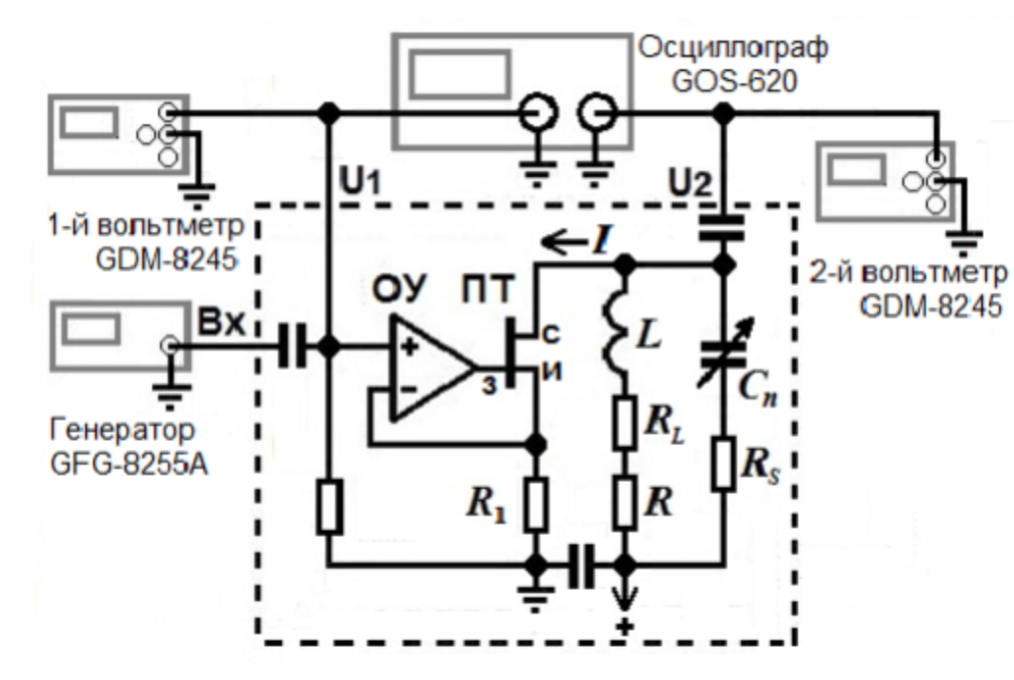
\includegraphics[width=0.4\textwidth]{im2.png}
    \caption{Последовательная эквивалентная схема конденсатора с потерями.}
    \label{pic:scheme2}
\end{figure}

Приступим к расчёту контура. Тогда ток на генераторе:
\[
    I=\dfrac{E}{R_I}=\dfrac{E_0cos(\omega t+\varphi_0)}{R_I}=I_0cos(\omega t+\varphi_0).
\]

\[
    R_S=\dfrac{U_{RS}}{I}=\frac{U_{RS}}{\omega CU_{CS}}=\dfrac{1}{\omega C}tg\delta,
\]
где $R_S$ - эквивалентное последовательное сопротивление (ЭПС).
Для используемых емкостей $C_n$ выполнено $tg\delta<10^{-3}$
\[
    R_{\sum}=R+R_L+R_S,
\]
где $R_{\sum}$ - суммарное активное сопротивление контура.
Воспользуемся методом комплексных амплитуд:
\[
    Z_L=R_L+i\omega L, \, Z_C=R_S-i\frac{1}{\omega C}, \, Z=R_{\sum}+i(\omega L-d\dfrac{1}{\omega C}).
\]
Тогда напряжение на контуре и токи на индуктивной и емкостной частях контура при нулевой начальной фазе можно предствить в виде:
\[
    I_c=I\dfrac{Z_L}{Z_C+Z_L}=iQI_0\dfrac{\omega}{\omega_0}\dfrac{1-i\dfrac{R+R_L}{\rho}\dfrac{\omega_0}{\omega}}{1+iQ(\dfrac{\omega}{\omega_0}-\dfrac{\omega_0}{\omega})},
\]
\[
    I_L=I\dfrac{Z_c}{Z_C+Z_L}=iQI_0\frac{\omega_0}{\omega}\frac{1+itg\delta}{1+iQ(\frac{\omega}{\omega_0}-\frac{\omega_0}{\omega})},
\]
\[
    U=I\frac{Z_LZ_c}{Z_C+Z_L}=Q\rho I_0\frac{(1-i\frac{R+R_L}{\rho}\frac{\omega_0}{\omega})(1+itg\delta)}{1+iQ(\frac{\omega}{\omega_0}-\frac{\omega_0}{\omega})},
\]
где $\omega_0=\frac{1}{\sqrt{LC}}$ - собственная частота, $\rho=\sqrt{\frac{L}{C}}$ - реактивное сопротивление контура, $Q=\frac{\rho} - {R_{\sum}}$ - добротность контура\newline
Рассмотрим случай, когда $|\Delta\omega|=|\omega-\omega_0|\ll\omega_0$. 
Тогда
\[
    \frac{\omega}{\omega_0}-\frac{\omega_0}{\omega}=\frac{2\Delta\omega}{\omega_0}.
\]
Пренебрегая поправками порядка $Q^{-2}$, получим:
\[
    I_c=QI_0\frac{\omega}{\omega_0}\frac{e^{i\phi_c}}{\sqrt{1+(\tau\Delta\omega)^2}}, \phi_c=\frac{\pi}{2}-\frac{R+R_L}{\rho}-arctg(\tau\Delta\omega),
\]
\[
    I_L=QI_0\frac{\omega_0}{\omega}\frac{e^{i\phi_L}}{\sqrt{1+(\tau\Delta\omega)^2}}, \phi_L=-\frac{\pi}{2}+\delta\arctg(\tau\Delta\omega),
\]
\[
    U=Q\rho I_0\frac{\omega}{\omega_0}\frac{e^{i\phi_U}}{\sqrt{1+(\tau\Delta\omega)^2}}, \phi_U=-\frac{\omega}{\omega_0}\frac{R+R_L}{\rho}+\delta-arctg(\tau\Delta\omega),
\]
где $\tau=\frac{2L}{R_{\sum}}=\frac{2Q}{\omega_0}$ - время затухания.\newline
При резонансе, т.е. когда $\Delta\omega=0$:
\[
    I_c(\omega_0)=QI_0, \phi_c(\omega_0)=\frac{\pi}{2}-\frac{R+R_L}{\rho},
\]
\[
    I_L(\omega_0)=QI_0, \phi_L(\omega_0)=-\frac{\pi}{2}+\delta,
\]
\[
    U(\omega_0)=Q\rho I_0=Q^2R_{\sum}I_0, \phi_U{\omega_0}=-\frac{R+R_L}{\rho}+\delta,
\]
\[
    \phi'_c(\omega_0)=\phi'_L(\omega_0)=\phi'_U(\omega_0)=-\tau.
\]

\section{Результаты и их обсуждение}
Результаты измерения резонансных частот схемы для различных ёмкостей конденсаторов $C$ и косвенные величины, вычисленные
из полученных значений представлены в таблице \ref{tab:1}. Значения величин, вычесленных косвенно были получены согласно формулам \ref{app_2}.
\begin{table}[H]
    \centering
    \begin{tabular}{|l|l|l|l|l|l|l|l|l|l|l|}
        \hline
        $C$, нФ & $f$, кГц & $U$, В & $E$, В & $L$, мГн & $\rho$ & $Z$, Ом & $Q$   & $R_{sum}$, Ом & $R_{smax}$, Ом & $R_L$, Ом \\ \hline
        25,1    & 32,12    & 1,45   & 0,25   & 978      & 197,4  & 5850,8  & 29,64 & 6,66          & 0,20           & 3,0       \\ \hline
        33,2    & 27,81    & 1,14   & 0,25   & 986      & 172,4  & 4593,3  & 26,65 & 6,47          & 0,17           & 2,8       \\ \hline
        47,3    & 23,21    & 0,82   & 0,25   & 994      & 145,0  & 3320,4  & 22,90 & 6,33          & 0,14           & 2,7       \\ \hline
        57,4    & 21,26    & 0,71   & 0,25   & 976      & 130,4  & 2852,2  & 21,87 & 5,96          & 0,13           & 2,3       \\ \hline
        67,5    & 19,47    & 0,57   & 0,25   & 990      & 121,1  & 2278,9  & 18,82 & 6,44          & 0,12           & 2,8       \\ \hline
        82,7    & 17,76    & 0,29   & 0,25   & 971      & 108,4  & 1179,0  & 10,88 & 9,96          & 0,11           & 2,3       \\ \hline
        101,6   & 16,06    & 0,42   & 0,25   & 967      & 97,5   & 1686,7  & 17,29 & 5,64          & 0,10           & 2,0       \\ \hline
        Ср знач & ~        & ~      & ~      & 980      & ~      & ~       & ~     & ~             & ~              & 2,6       \\ \hline
        Погр    & ~        & ~      & ~      & 4        & ~      & ~       & ~     & ~             & ~              & 0,5       \\ \hline
    \end{tabular}
    \caption{Результаты измерения резонансных частот $f$ при разных значениях ёмкостей конденсаторов $C$ при
        напряжении на схеме $E$. $U$ --- напряжение на конденсаторе, $L$ --- индуктивность катушки, $\rho$ --- харастеристика
        активного сопростивления конденсатора, $Z$ --- модуль импеданса контура, $Q$ --- добротность контура,
        $R_{sum}$ --- полное активное сопротивление контура, $R_{smax}$ --- максимальное активное сопротивление конденсатора,
        $R_L$ --- активное сопротивление катушки.
    }
    \label{tab:1}
\end{table}

Измерены зависимости напряжения на конденсаторе от частоты вблизи резонанса ($U \geq 0.6 U_0$) для конденсаторов
с номерами 3 и 5 (Таблицы \ref{tab:2} и \ref{tab:3}). Построены АЧХ для соответствующий конденсаторов (Рис. \ref{fig:Uf}).

\begin{figure}
    \centering
    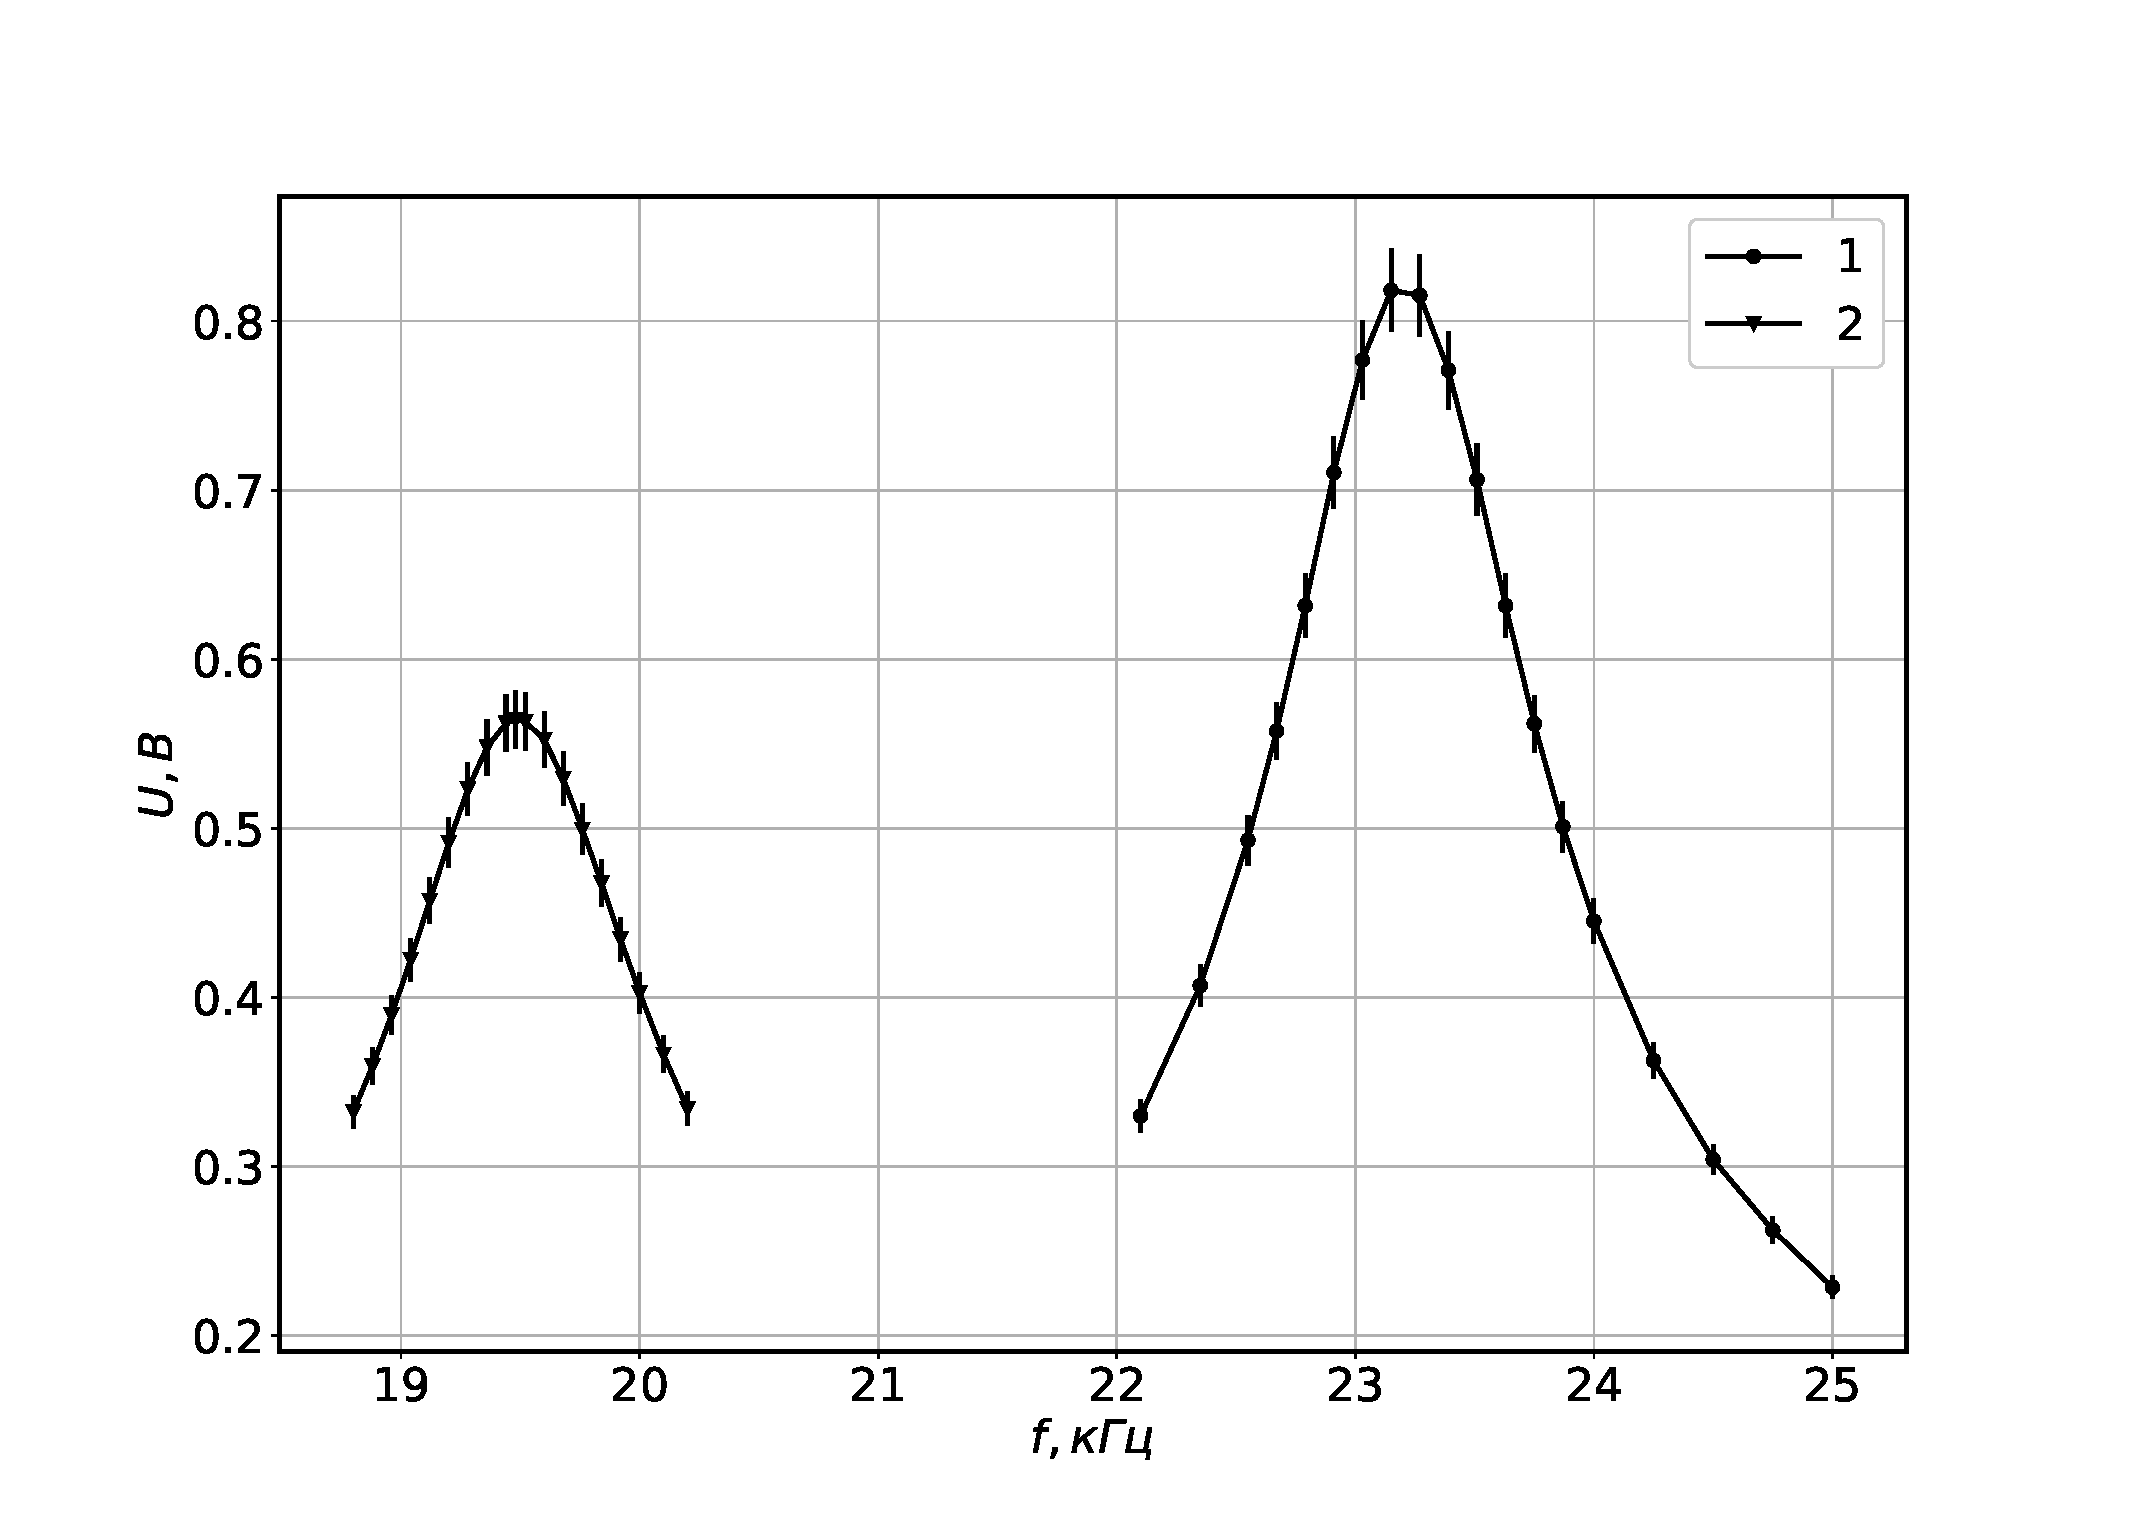
\includegraphics[width=0.7\textwidth]{Uf.eps}
    \caption{Зависимость напряжения на конденсаторе $U$ от частоты $f$ вблизи резонанса. 1 --- АЧХ для конденсатора
        с $C = 47,3$ нФ, 2 --- АЧХ для конденсатора с $C = 67,5$ нФ.}
    \label{fig:Uf}
\end{figure}

Согласно приведённым графикам при меньшей ёмкости конденсатора $C$ резонанс достигается при большей частоте и большей амплитуде напряжения.
Для лучшего анализа построены АЧХ в нормированных осях $\frac{U}{U_0}\left( \frac{f}{f_0} \right) $ (Рис. \ref{fig:Uf_norm}).

\begin{figure}
    \centering
    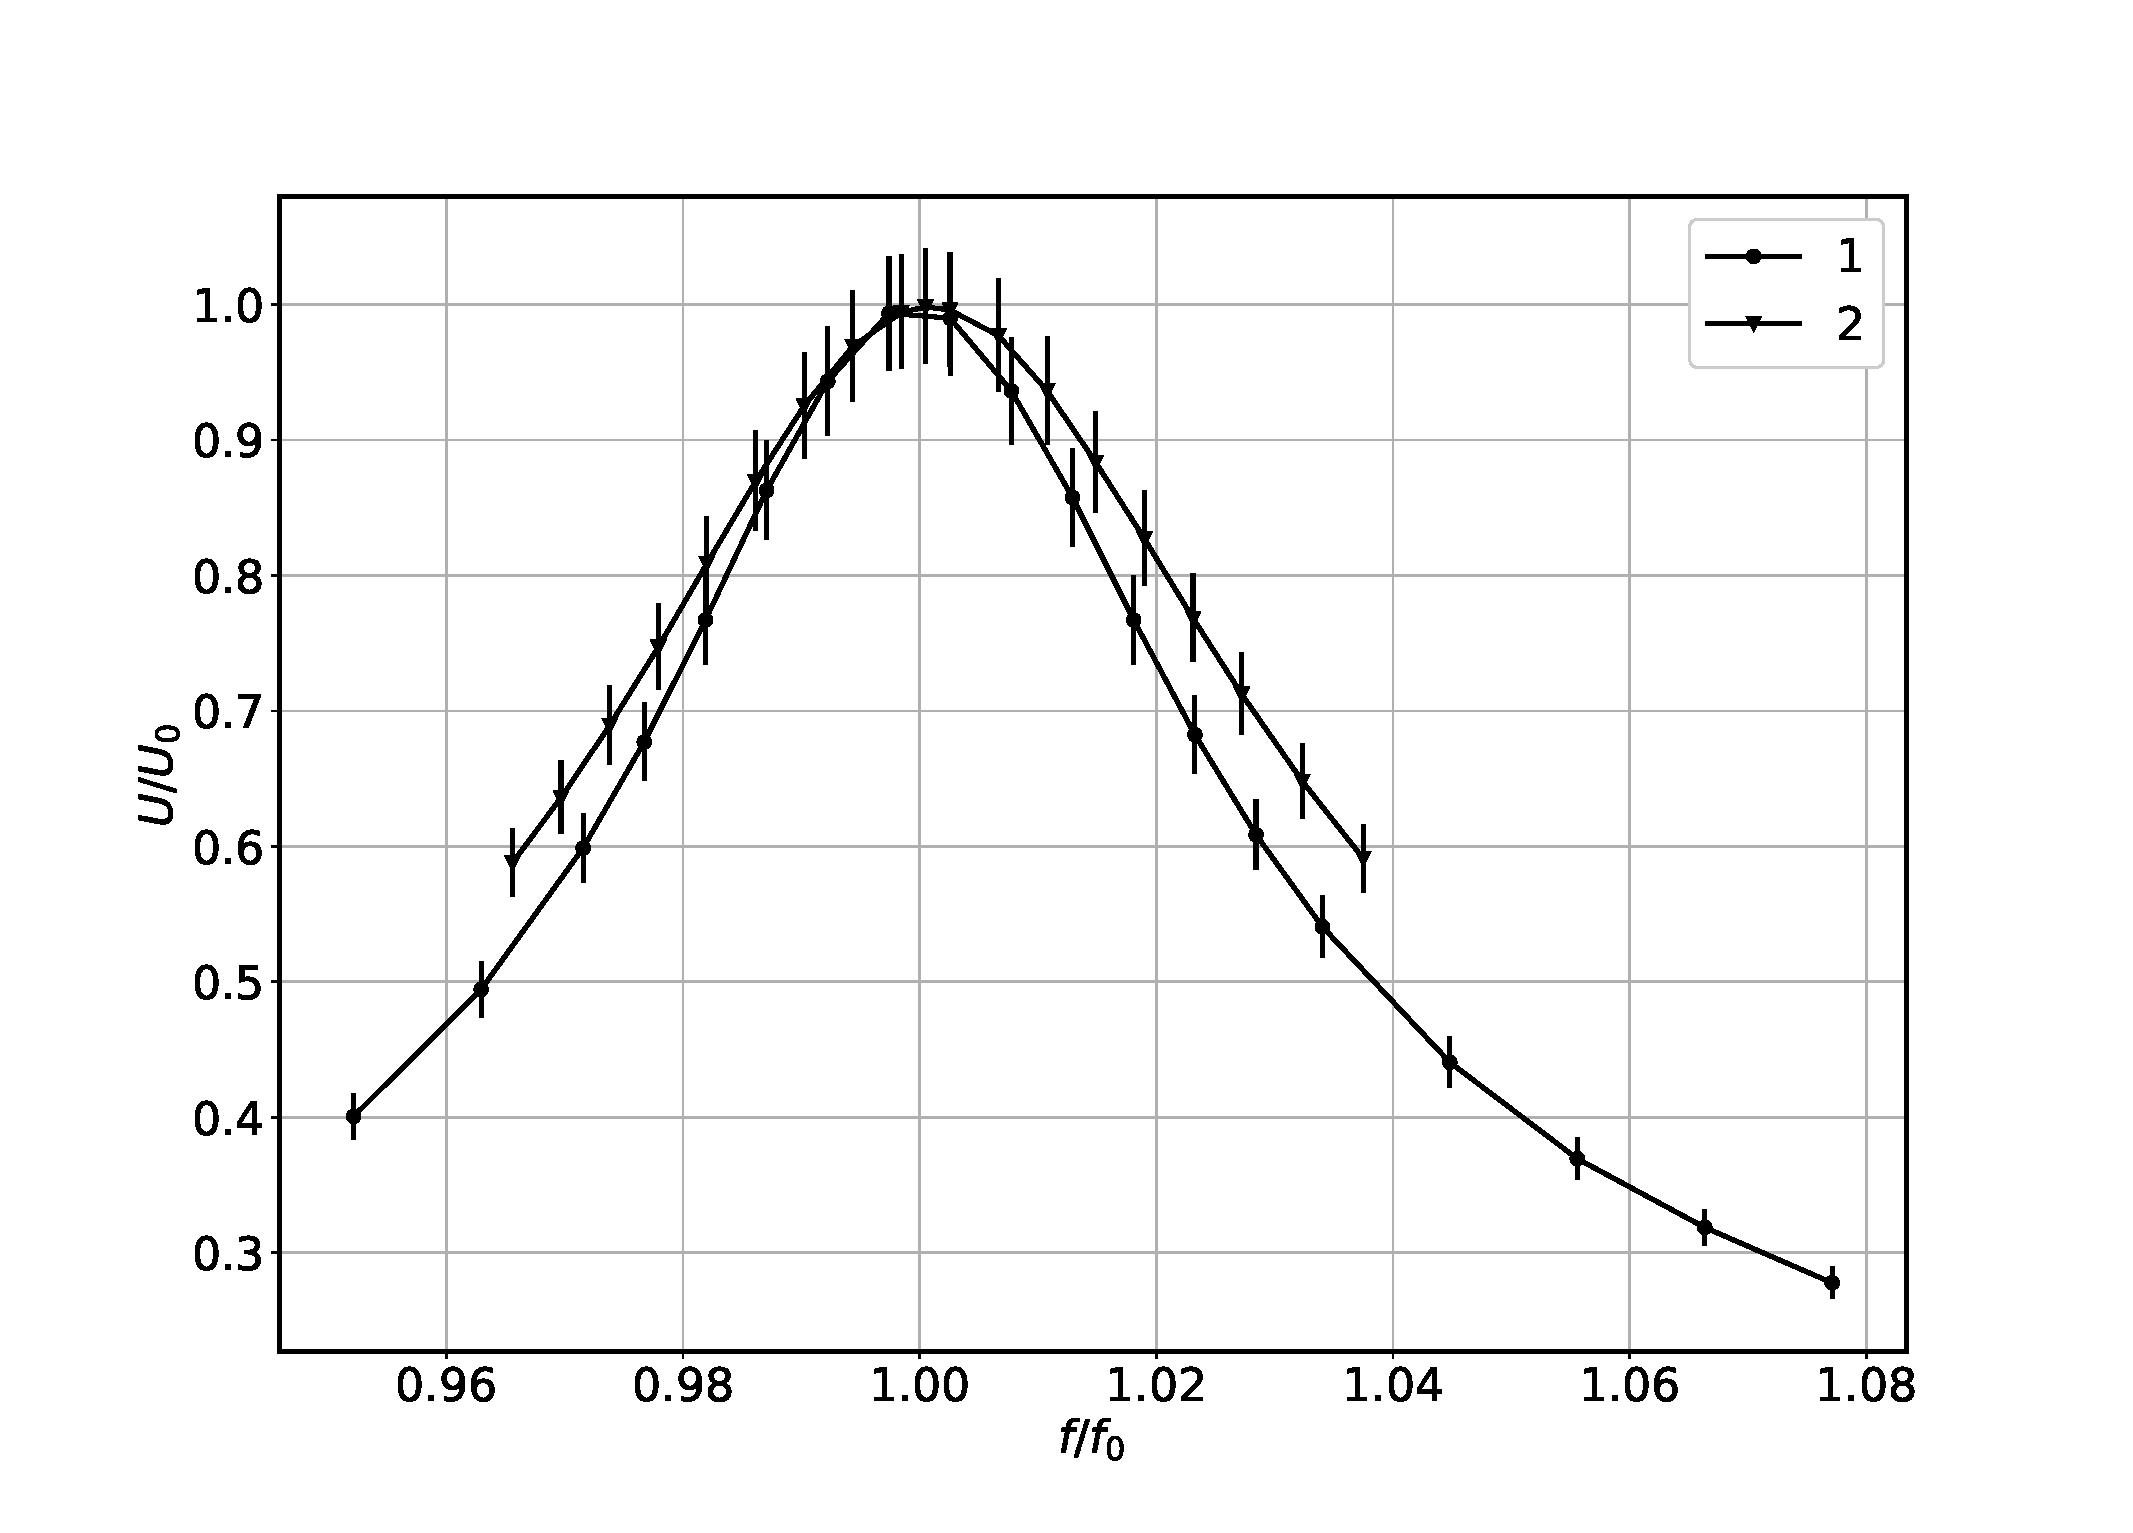
\includegraphics[width=0.7\textwidth]{Uf_norm.eps}
    \caption{Зависимость нормированного напряжения на конденсаторе $\frac{U}{U_0}$ от нормированной частоты $\frac{f}{f_0}$ вблизи резонанса.
        1 --- АЧХ для конденсатора с $C = 47,3$ нФ, 2 --- АЧХ для конденсатора с $C = 67,5$ нФ.}
    \label{fig:Uf_norm}
\end{figure}

По ширине нормированной АЧХ на высоте $\frac{U}{U_0} = \sqrt{2}$ найдены значения добротности контуров $Q = \frac{w_0}{\Delta w}$.
Для цепи с конденсатором 3 $Q_3 \approx 23 \pm 1$, для цепи с конденсатором 5 $Q_5 \approx 19 \pm 1$. Что совпадает с добротностями,
рассчитанных из резонанса (Таблица \ref{tab:1}) $Q_{3t} = 22,9$, $Q_{5t} = 18,82$.

Измерена зависимость фазы на конденсаторе в зависимости от частоты вблизи резонанса для конденсаторов 3 и 5(Таблицы \ref{tab:4} и \ref{tab:5}).
Построен график нормированной ФЧХ(Рис. \ref{fig:pf}). Расстоянию между точками $\frac{\varphi}{\varphi_0} = -\frac{1}{4}, \frac{1}{4}$ получим
добротность. $Q_3 = 22,8 \pm 0,5$, $Q_5 = 18,7 \pm 0,5$, что совпадает с предыдущими рассчитанными значениями добротностями контуров.

\begin{figure}
    \centering
    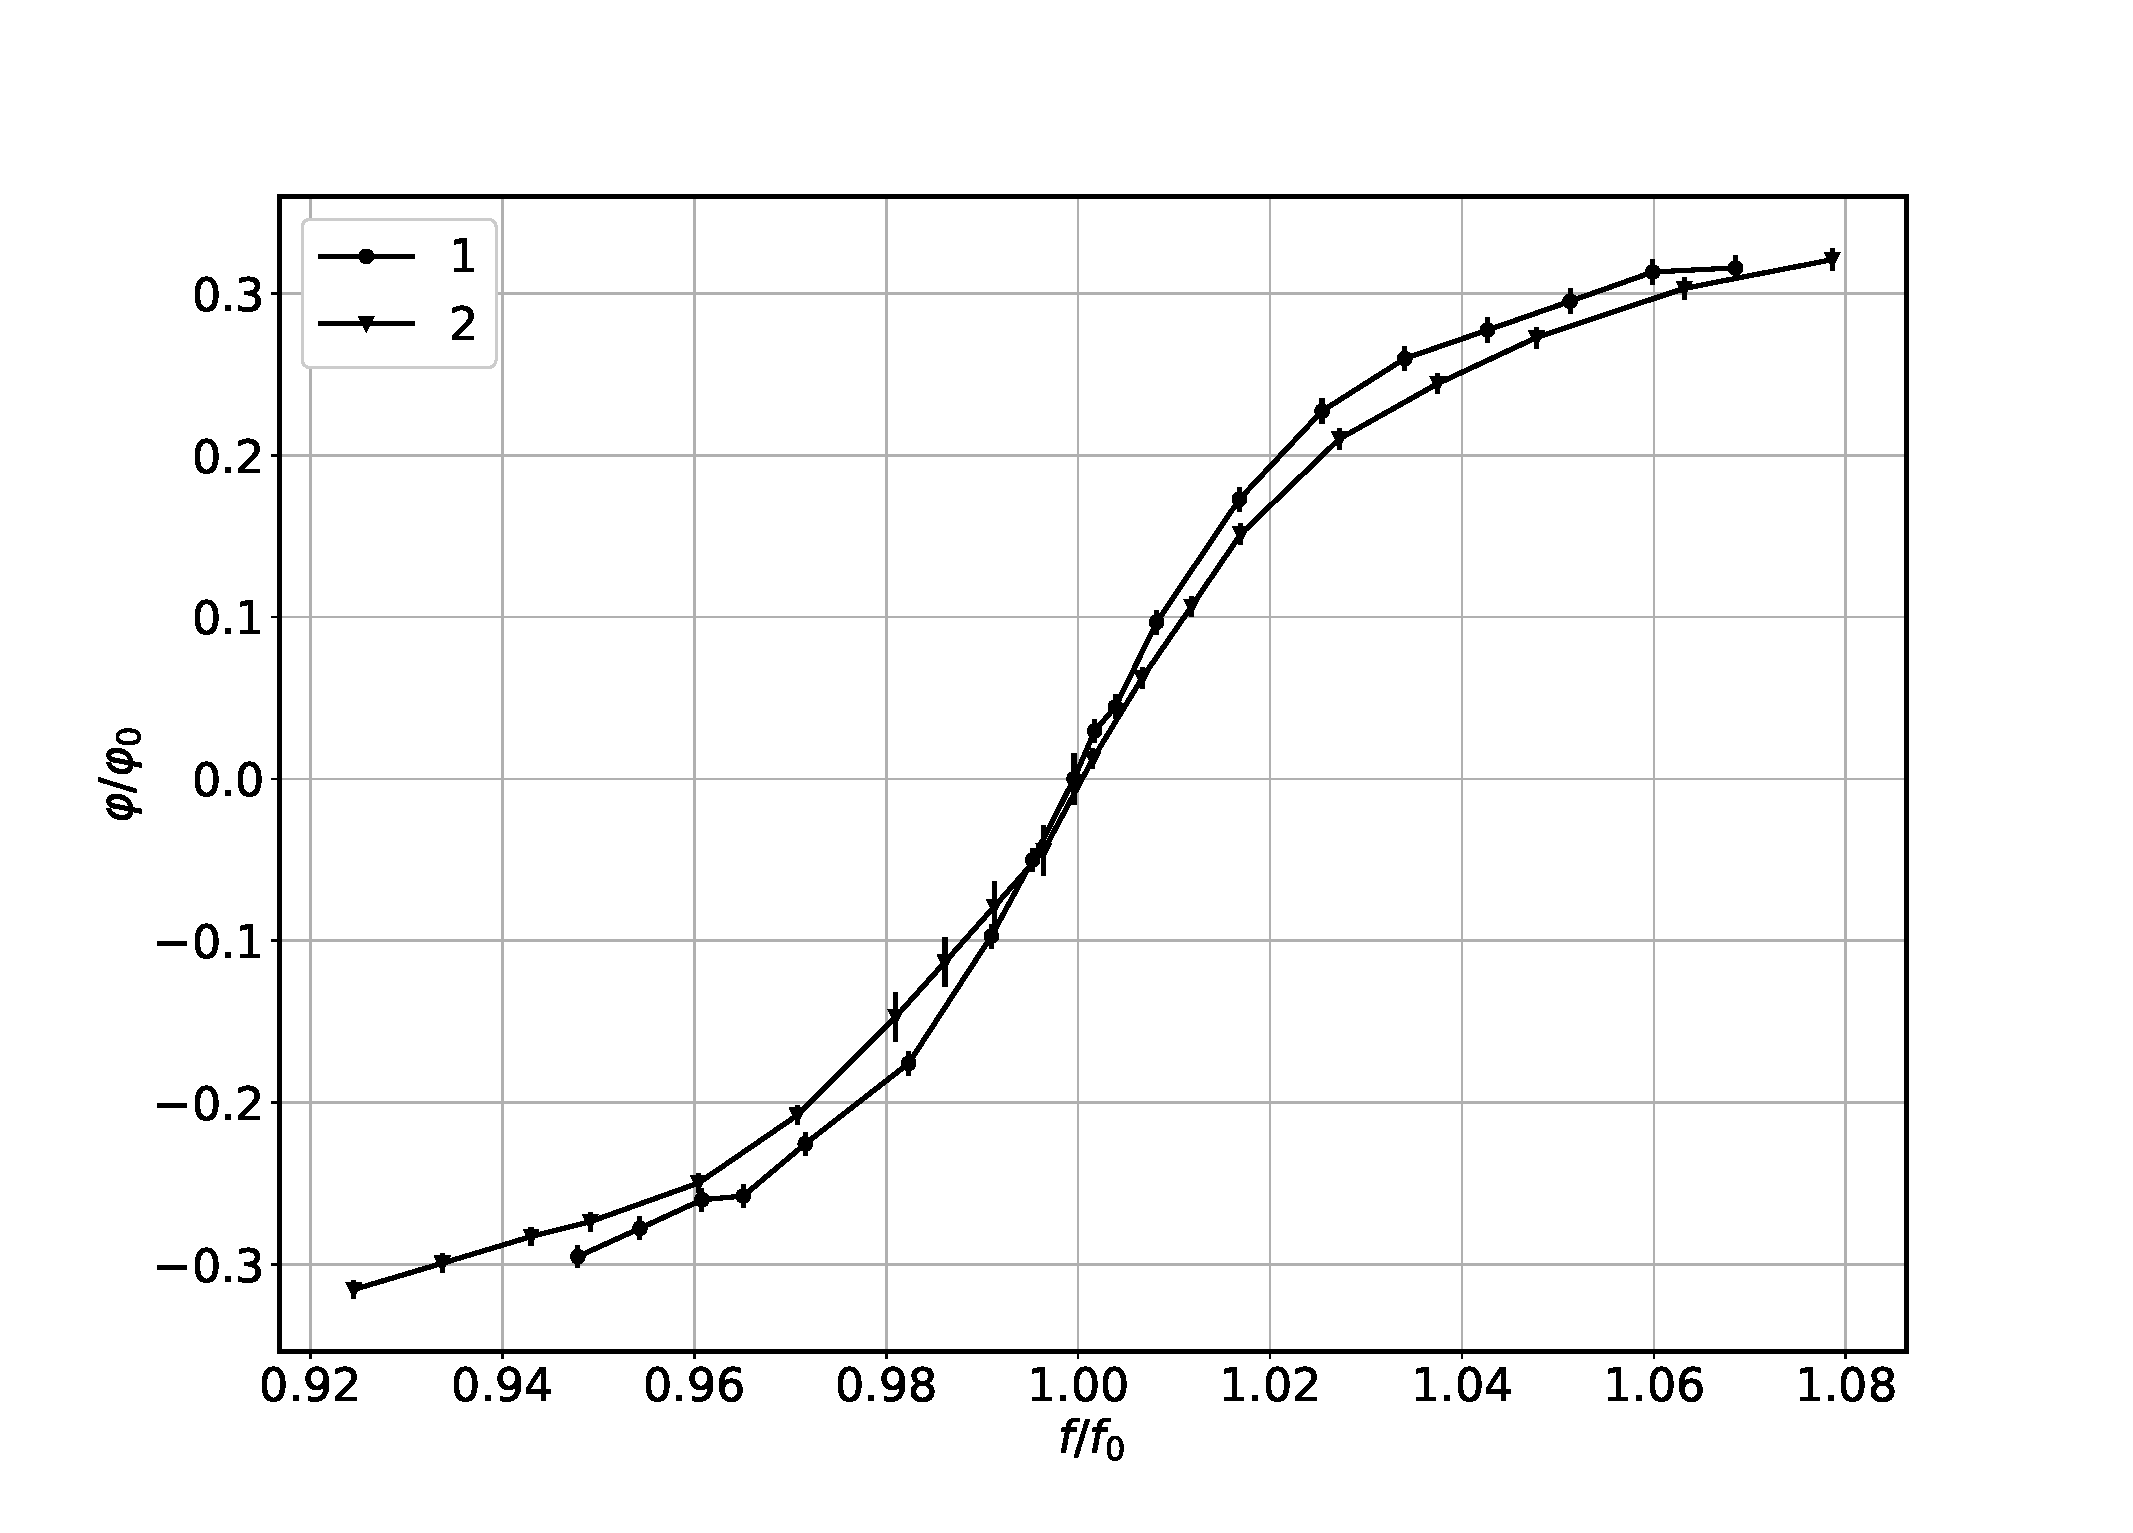
\includegraphics[width=0.7\textwidth]{pf_norm.eps}
    \caption{Зависимость нормированной фазы на конденсаторе $\frac{\varphi}{\varphi_0}$ от нормированной частоты $\frac{f}{f_0}$ вблизи резонанса. 1 --- ФЧХ для конденсатора
        с $C = 47,3$ нФ, 2 --- ФЧХ для конденсатора с $C = 67,5$ нФ.}
    \label{fig:pf}
\end{figure}

\begin{figure}
    \centering
    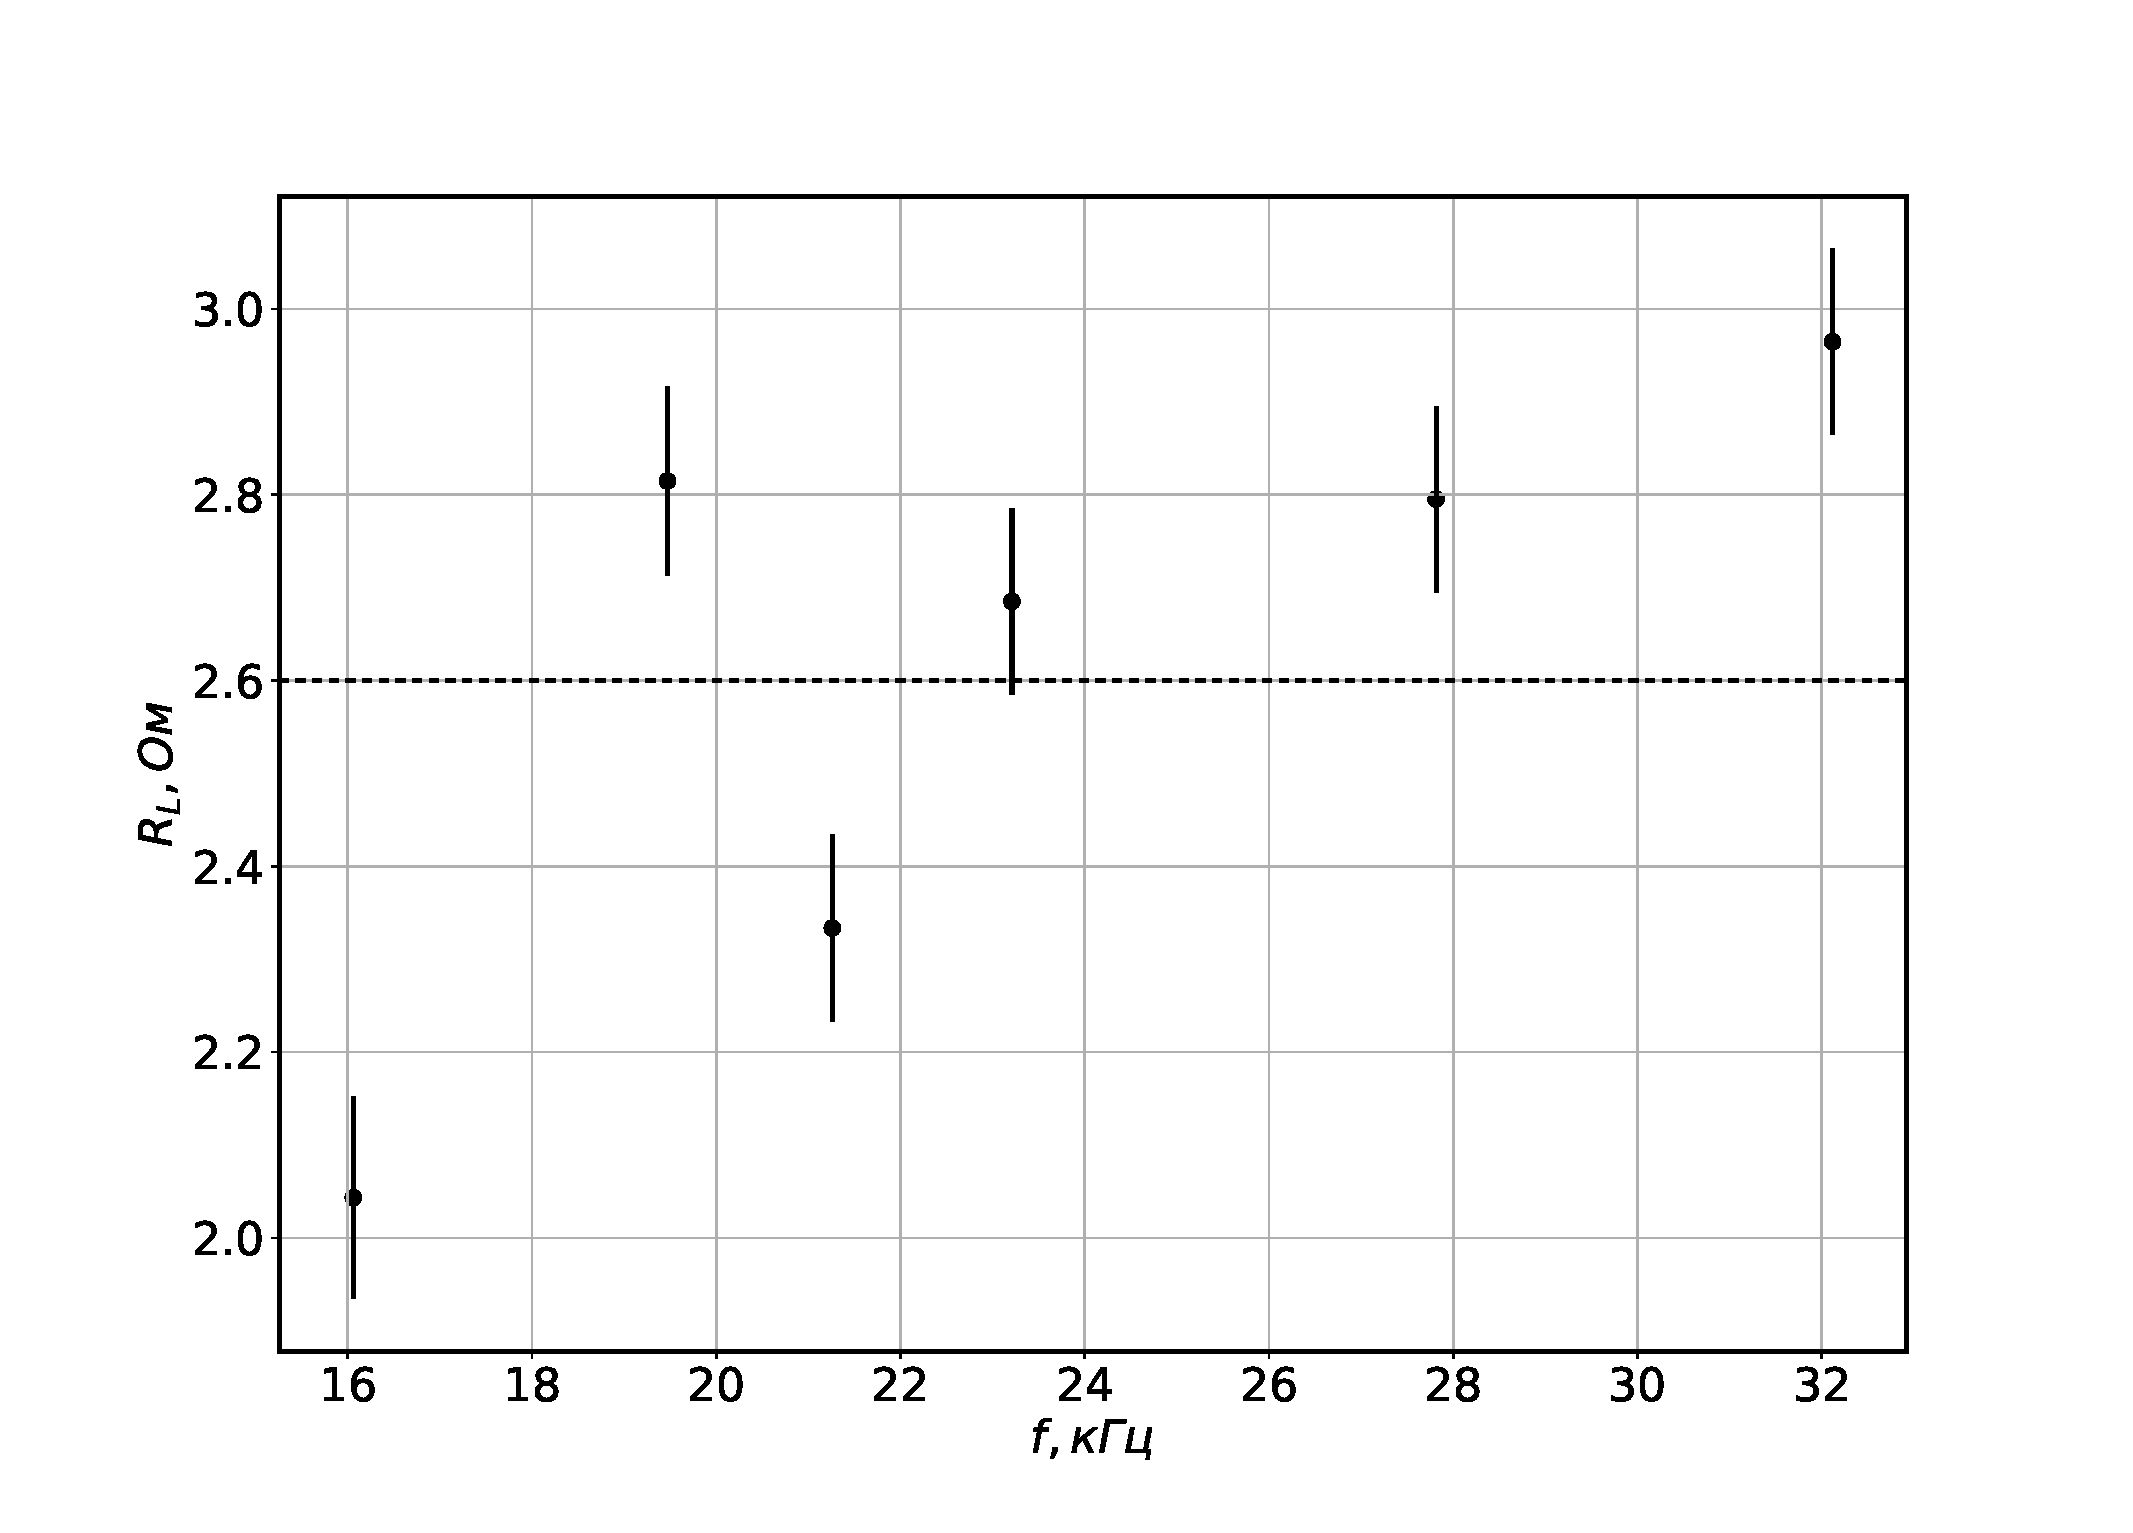
\includegraphics[width=0.7\textwidth]{RLf.eps}
    \caption{Зависимость активного сопротивления катушки $R_L$ от резонансных частот $f$. Пунктиром обозначено
        среднее значение сопротивлений.}
    \label{fig:RLf}
\end{figure}

\section{Выводы}
Исследован резонанс токов в параллельном колебательном контуре с изменяемой
ёмкостью, включающее получение амплитудно-частотных и фазово-частотных характеристик, 
а также определение основных параметров контура.
Определена добротность контуров с помощью непосредственных измерений резонанса, графиков АЧХ
и ФЧХ, полученные результаты совпали в пределах погрешности. 


\section{Использованная литература}
\begin{thebibliography}{9}
    \bibitem{LabBook}
    Лабораторный практикум по общей физике, Том 2, под редакцией А. Д. Гладуна
\end{thebibliography}

\section{Приложения}
\subsection{Параметры установки и погрешности приборов} \label{app_1}
Сопротивления установки, представленной на Рис. \ref{pic:scheme2}: $R_1 = 1008$, $R = 3,5$ Ом.
Погрешность вольтметра $3\%$.

\subsection{Формулы для расчёта параметров контура} \label{app_2}
\begin{equation}\label{}
    L=\frac{1}{C(2\pi f)^2} \\
\end{equation}
\begin{equation}\label{}
    \rho=\frac{1}{2\pi fC} \\
\end{equation}
\begin{equation}\label{}
    Z_{\text{рез}}=\frac{U}{E_0}R_1
\end{equation}
\begin{equation}\label{}
    Q=\frac{UR_1}{E_0}2\pi fC
\end{equation}
\begin{equation}\label{}
    R_{\sum}=\frac{E_0}{UR_1}\frac{1}{(2\pi fC)^2}
\end{equation}
\begin{equation}\label{}
    R_{Smax}=10^{-3}\cdot\frac{1}{\omega_0C}
\end{equation}
\begin{equation}\label{}
    R_L=\frac{E_0}{UR_1}\frac{1}{(2\pi fC)^2}-R-10^{-3}\cdot\frac{1}{\omega_0C}
\end{equation}

\subsection{Данные результатов измерений} \label{app_3}
\begin{table}[H]
    \centering
    \begin{tabular}{|l|l|l|l|}
        \hline
        $f$, кГц & $U$, В & $\sigma f$, кГц & $\sigma U$, кГц \\ \hline
        22,100   & 0,33   & 0,001           & 0,01            \\ \hline
        22,350   & 0,41   & 0,001           & 0,01            \\ \hline
        22,550   & 0,49   & 0,001           & 0,01            \\ \hline
        22,670   & 0,56   & 0,001           & 0,02            \\ \hline
        22,790   & 0,63   & 0,001           & 0,02            \\ \hline
        22,910   & 0,71   & 0,001           & 0,02            \\ \hline
        23,030   & 0,78   & 0,001           & 0,02            \\ \hline
        23,150   & 0,82   & 0,001           & 0,02            \\ \hline
        23,270   & 0,82   & 0,001           & 0,02            \\ \hline
        23,390   & 0,77   & 0,001           & 0,02            \\ \hline
        23,510   & 0,71   & 0,001           & 0,02            \\ \hline
        23,630   & 0,63   & 0,001           & 0,02            \\ \hline
        23,750   & 0,56   & 0,001           & 0,02            \\ \hline
        23,870   & 0,50   & 0,001           & 0,02            \\ \hline
        24,000   & 0,45   & 0,001           & 0,01            \\ \hline
        24,250   & 0,36   & 0,001           & 0,01            \\ \hline
        24,500   & 0,30   & 0,001           & 0,01            \\ \hline
        24,750   & 0,26   & 0,001           & 0,01            \\ \hline
        25,000   & 0,23   & 0,001           & 0,01            \\ \hline
    \end{tabular}
    \caption{Результаты измерения зависимости напряжения на конденсаторе $U$ от частоты $f$ в близи резонанса.
        Ёмкость конденсатора $C = 47,3$ нФ.}
    \label{tab:2}
\end{table}

\begin{table}[H]
    \centering
    \begin{tabular}{|l|l|l|l|}
        \hline
        $f$, кГц & $U$, В & $\sigma f$, кГц & $\sigma U$, кГц \\ \hline
        18,800   & 0,33   & 0,001           & 0,01            \\ \hline
        18,880   & 0,36   & 0,001           & 0,01            \\ \hline
        18,960   & 0,39   & 0,001           & 0,01            \\ \hline
        19,040   & 0,42   & 0,001           & 0,01            \\ \hline
        19,120   & 0,46   & 0,001           & 0,01            \\ \hline
        19,200   & 0,49   & 0,001           & 0,01            \\ \hline
        19,280   & 0,52   & 0,001           & 0,02            \\ \hline
        19,360   & 0,55   & 0,001           & 0,02            \\ \hline
        19,440   & 0,56   & 0,001           & 0,02            \\ \hline
        19,480   & 0,56   & 0,001           & 0,02            \\ \hline
        19,520   & 0,56   & 0,001           & 0,02            \\ \hline
        19,600   & 0,55   & 0,001           & 0,02            \\ \hline
        19,680   & 0,53   & 0,001           & 0,02            \\ \hline
        19,760   & 0,50   & 0,001           & 0,01            \\ \hline
        19,840   & 0,47   & 0,001           & 0,01            \\ \hline
        19,920   & 0,43   & 0,001           & 0,01            \\ \hline
        20,000   & 0,40   & 0,001           & 0,01            \\ \hline
        20,100   & 0,37   & 0,001           & 0,01            \\ \hline
        20,200   & 0,33   & 0,001           & 0,01            \\ \hline
    \end{tabular}
    \caption{Результаты измерения зависимости напряжения на конденсаторе $U$ от частоты $f$ в близи резонанса.
        Ёмкость конденсатора $C = 67,5$ нФ.}
    \label{tab:3}
\end{table}


\begin{table}[H]
    \centering
    \begin{tabular}{|l|l|l|l|}
        \hline
        $f$, кГц & $\varphi$ & $f$, кГц & $\sigma \varphi$ \\ \hline
        22,000   & 1,54      & 0,001    & 0,02             \\ \hline
        22,150   & 1,59      & 0,001    & 0,02             \\ \hline
        22,300   & 1,65      & 0,001    & 0,02             \\ \hline
        22,400   & 1,66      & 0,001    & 0,02             \\ \hline
        22,550   & 1,76      & 0,001    & 0,02             \\ \hline
        22,800   & 1,92      & 0,001    & 0,02             \\ \hline
        23,000   & 2,16      & 0,001    & 0,02             \\ \hline
        23,100   & 2,31      & 0,001    & 0,02             \\ \hline
        23,200   & 0,00      & 0,001    & 0,05             \\ \hline
        23,250   & 0,09      & 0,001    & 0,02             \\ \hline
        23,300   & 0,14      & 0,001    & 0,02             \\ \hline
        23,400   & 0,30      & 0,001    & 0,02             \\ \hline
        23,600   & 0,54      & 0,001    & 0,02             \\ \hline
        23,800   & 0,71      & 0,001    & 0,02             \\ \hline
        24,000   & 0,82      & 0,001    & 0,02             \\ \hline
        24,200   & 0,87      & 0,001    & 0,02             \\ \hline
        24,400   & 0,93      & 0,001    & 0,02             \\ \hline
        24,600   & 0,98      & 0,001    & 0,02             \\ \hline
        24,800   & 0,99      & 0,001    & 0,02             \\ \hline
    \end{tabular}
    \caption{Результаты измерения зависимости фазы на конденсаторе $\varphi$ от частоты $f$ в близи резонанса.
        Ёмкость конденсатора $C = 47,3$ нФ.}
    \label{tab:4}
\end{table}


\begin{table}[H]
    \centering
    \begin{tabular}{|l|l|l|l|}
        \hline
        $f$, кГц & $\varphi$ & $f$, кГц & $\sigma \varphi$ \\ \hline
        18,000   & 1,48      & 0,001    & 0,02             \\ \hline
        18,180   & 1,53      & 0,001    & 0,02             \\ \hline
        18,360   & 1,58      & 0,001    & 0,02             \\ \hline
        18,480   & 1,61      & 0,001    & 0,02             \\ \hline
        18,700   & 1,68      & 0,001    & 0,02             \\ \hline
        18,900   & 1,81      & 0,001    & 0,02             \\ \hline
        19,100   & 2,01      & 0,001    & 0,05             \\ \hline
        19,200   & 2,11      & 0,001    & 0,05             \\ \hline
        19,300   & 2,22      & 0,001    & 0,05             \\ \hline
        19,400   & 2,33      & 0,001    & 0,05             \\ \hline
        19,500   & 0,04      & 0,001    & 0,02             \\ \hline
        19,600   & 0,20      & 0,001    & 0,02             \\ \hline
        19,700   & 0,33      & 0,001    & 0,02             \\ \hline
        19,800   & 0,48      & 0,001    & 0,02             \\ \hline
        20,000   & 0,66      & 0,001    & 0,02             \\ \hline
        20,200   & 0,77      & 0,001    & 0,02             \\ \hline
        20,400   & 0,86      & 0,001    & 0,02             \\ \hline
        20,700   & 0,95      & 0,001    & 0,02             \\ \hline
        21,000   & 1,01      & 0,001    & 0,02             \\ \hline
    \end{tabular}
    \caption{Результаты измерения зависимости фазы на конденсаторе $\varphi$ от частоты $f$ в близи резонанса.
        Ёмкость конденсатора $C = 67,5$ нФ. Повышение погрешности вблизи резонанса связано с изменением режима
        просмотра на осцилографе.}
    \label{tab:5}
\end{table}


\end{document}